\documentclass[a4paper]{article}
\usepackage{geometry}
\geometry{a4paper, portrait, margin=1in}
\usepackage[english]{babel}
\usepackage[utf8]{inputenc}
\usepackage{natbib}
\usepackage{graphicx}
\usepackage{fancyhdr}
\usepackage{array}
\usepackage{tabu}
\usepackage{listings}
\usepackage[export]{adjustbox}

\title{Computing GCSE Coursework}
\author{\\ \\ \\ \\ Thomas Bass\\Candidate 4869\\Centre 52423\\OCR A452 Practical Investication\\\\Made with \LaTeX}
\date{2017}


\pagestyle{fancy}
\fancyhf{}
\rhead{Computing GCSE Coursework}
\chead{Candidate 4869}
\lhead{Thomas Bass}
\rfoot{Page \thepage}

\begin{document}

\maketitle
\pagebreak
\renewcommand*\contentsname{Summary}
\tableofcontents
\pagebreak

%%%%%%%%%%%%%%%%%%%%%%%%%%%%%%%%%%%%%%%%%%%%%%%%%%%%%%%%%%%%%%%%%%%%%%%%%

\section{Task 1}
Often, a web designer wants a change to happen when a user clicks on a screen object or moves the mouse over it. JavaScript can make changes to the HTML elements. \par
\noindent Enter and run this script: \par \par
\begin{lstlisting}
<!DOCTYPE html>
<html>
<body>
<h1>Change an HTML element</h1>
<p id="msg">Now you see me.</p>
<button type="button"
onclick="document.getElementById('msg').innerHTML = 'Gone!'">
Click Me!</button>
<button type="button"
onclick="document.getElementById('msg').innerHTML = 'Back again!'">
Bring me back!</button>
</body>
</html>
\end{lstlisting}
	

\subsection{Explain how you ran this script:} ~\par	

This script was copied into a HTML document, and opened into a web browser. 

When the script ran it gave the following output: ~\par ~\par
\noindent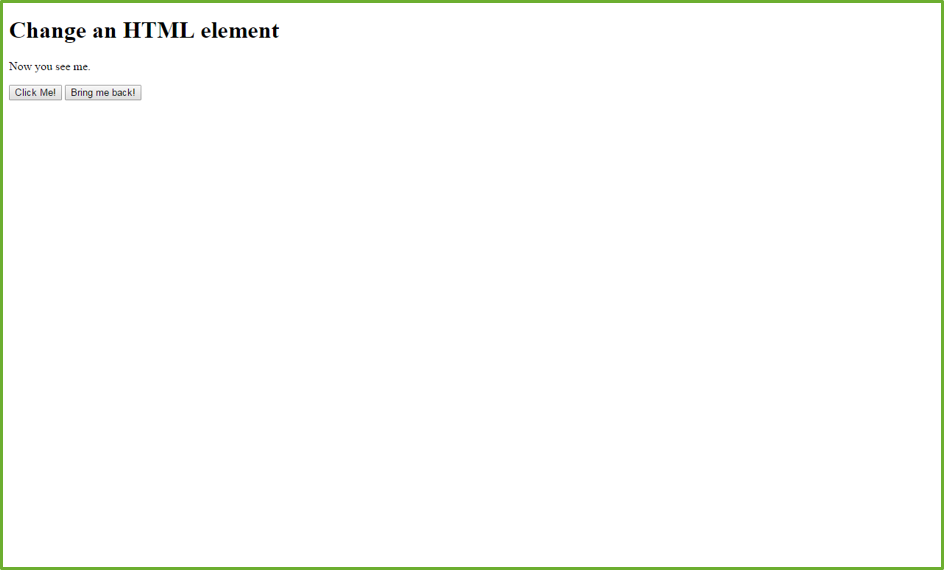
\includegraphics{Picture1.png} \par 

The web page took the code entered, ran it, and produced this output.











\end{document}